\section{Empirical Results}\label{sec:results}

\subsection{Data}\label{subsec:data}
In the empirical analysis, we analyse the capability 
of CME Bitcoin Futures (BTCF) to reduce the risk of
five cryptos, namely Bitcoin (BTC), Ethereum 
(ETH), Cardano (ADA), Litecoin (LTC) and Ripple (XRP), as well as five
crypto indexes, namely BITX, BITW100, CRIX, BITW20 and BITW70.
The currencies ETH, ADA, LTC, and XRP are popular cryptos traded at
various exchanges and have large market capitalization. 
BITX, BITW100, and CRIX are market-cap weighted crypto indexes with
BTC as constituent. 
BITX and BITW100 track the total return of the 10 and 100 cryptos
with largest market-cap, respectively. 
CRIX determines the number of constituents via AIC and tracks this
number of cryptos with largest market-cap. In our case, the number of
constituents in the CRIX is 5. 
BITW20 is also a market-cap weighted crypto index but with the 20
largest market-cap cryptos outside the constituents of BITX.
BITW70 has the same construction as BITW20 but with the 70 largest
market-cap cryptos outside BITX and BITW20. 
Therefore, BTC is excluded as a constituent in BITW20 and BITW70.

For each of the ten hedge portfolios, a crypto or index is considered
as the spot and held in a unit size long position, while 
the front BTCF is held in a short position with units corresponding to
the optimal hedge ratio in order to reduce the risk of the spot. 
Except for the hedge of BTC, all hedging portfolios are considered to
be cross-asset hedges. 

We collect the spots' and BTCF's daily prices at 15:00 US Central Time
(CT). The reason for choosing this particular time is that the CME
group determines the daily settlements for BTCF's based on the trading
activities on CME Globex between 14:59 and 15:00 CT. This is also the
reporting time of the daily closing price by Bloomberg. 
The crypto spot data is collected from the data provider called
Tiingo (\href{https://www.tiingo.com/}{https://www.tiingo.com/}).
Tiingo aggregates crypto OHLC (open, high, low, and close) prices fed
by APIs from various exchanges. It covers major exchanges, such as
Binance, Gemini, Poloniex, so Tiingo's aggregated OHLC price is a
reasonable representation of a tradable market price. 
For each crypto, we match the opening price at 15:00 CT from Tiingo
with the daily BTCF closing price from Bloomberg.
Since CRIX is not available at 15:00 CT, we recalculated an hourly
CRIX using the monthly constituents weights and the hourly OHLC price
data collected from Tiingo. 
BITX, BITW20, BITW70, and BITW100 are collected from the official
website of their publisher Bitwise.com. 
The daily reporting time of the Bitwise indexes is 15:00 CT.

The date range of the whole dataset is from 2018-08-13 to 2021-05-27. 

% At the time of writing, the CRIX is undergoing the listing process on
% the S\&P Dow Jones Indices. The official CRIX data will then be
% calculated with Lukka Prime Data and available to the public via
% S\&P. \natp{\em [Is this still the case?]}

\subsection{Overview of the out-of-sample data}\label{subsec:oosdata}

The date range of the out-of-sample time series is from 2019-10-21 to
2021-05-27, in total of 405 data points in each time series. 
This section gives an overview of the out-of-sample period. 

Figure~\ref{fig:BTC_price} presents the BTC and BTCF price in USD in
the first panel and the difference between the daily returns of BTC and BTCF,
 i.e. $R_s - R_f$, in the second panel. 
In the first panel, the black vertical lines with capital letters
labels indicate the days of the five most negative daily BTC returns
during out-pf-sample period.
Table \ref{tab:BTC_5min} summarizes the relevant news headlines and
events of those days.  

Figures~\ref{fig:index_price} and \ref{fig:individualCoins_price} show
the cumulative returns of the indices and individual cryptos,
respectively.  The vertical lines labeled by assets name refer to the 
largest daily price drops of each asset in the out-of-sample data.  
Table \ref{tab:All_min} summarises the events that are associated with largest prices drops in 
out-of-sample data. 

The out-of-sample data covers the pre-COVID19 period, 2019-10-21 to
2020-03-11 \footnote{See WHO's announcement in the media briefing on 2020-03-11 \url{https://www.who.int/director-general/speeches/detail/who-director-general-s-opening-remarks-at-the-media-briefing-on-covid-19---11-march-2020}.}, as well as the COVID19 period, 2019-03-11 onwards. 
We observe an overall upward trend of crypto prices in both periods.
Nonetheless, the volatilities of assets are high (annualized around
100\%) regardless of the COVID19 outbreak. 

\newpage
\begin{figure}[t]
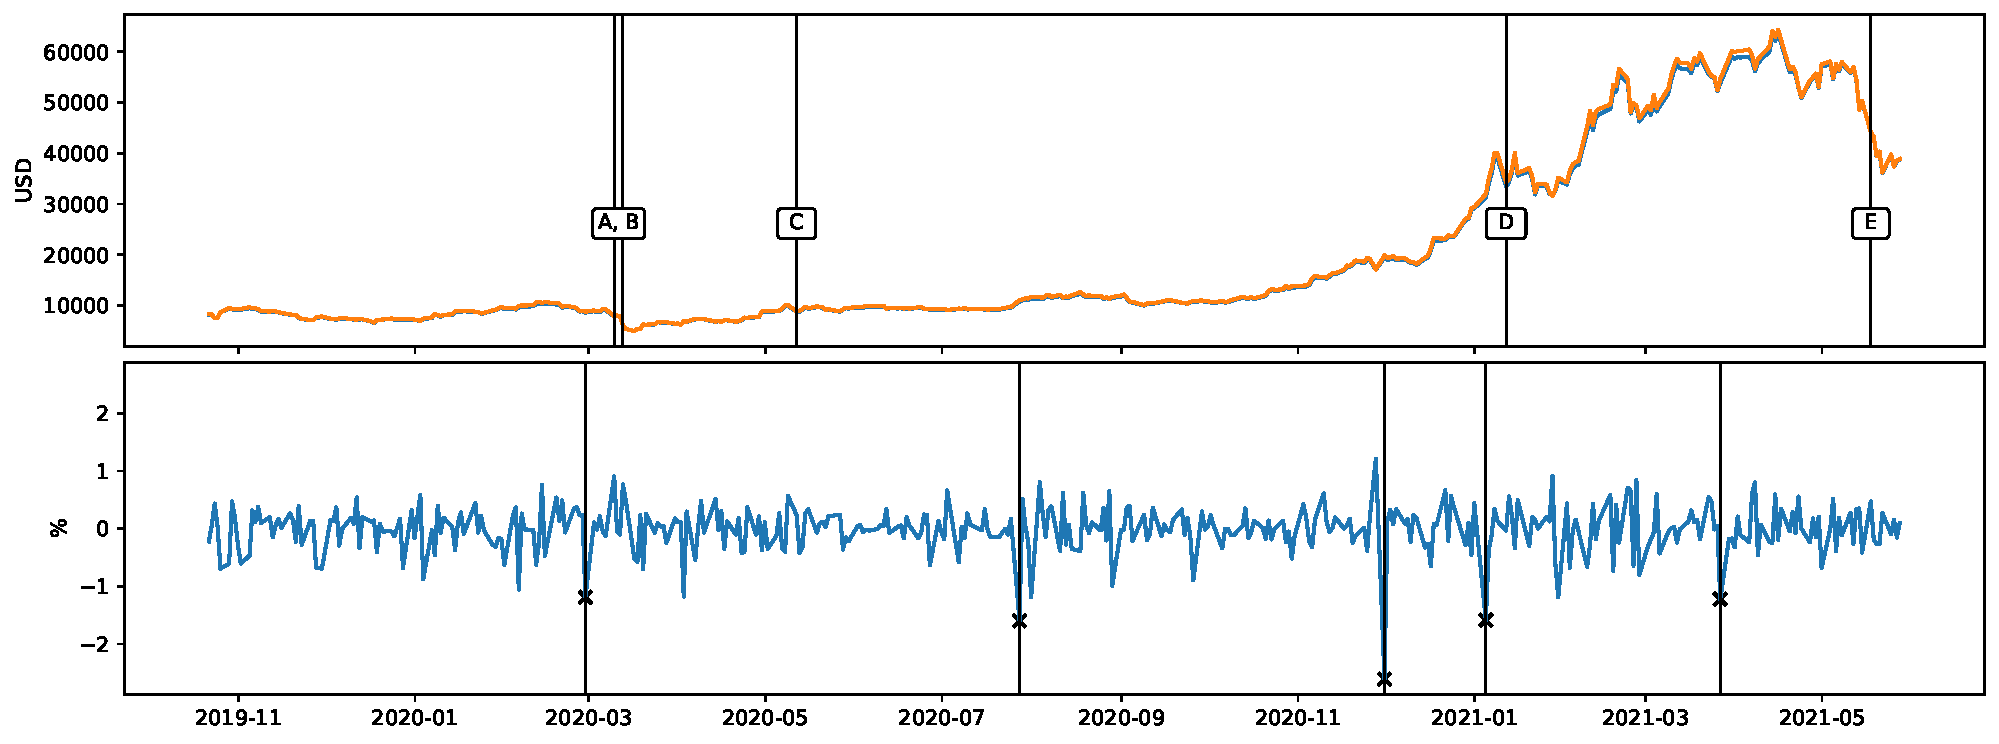
\includegraphics[width=\textwidth]{_pics/BTC_price.pdf}
  \caption{Out-of-sample BTC and BTCF price. The first panel presents the price of BTC in blue line and that of BTCF in orange line.
  The black vertical lines with capital letter labels indicate the five most negative daily return of BTC in the out-of-sample data.
  The second panel presents the difference between the percentage returns of BTC and BTCF.
  The black vertical lines indicate the five most negative returns.
  The crosses locate the level the returns.}
%  \href{http://www.quantlet.com/}{\includegraphics[height=\baselineskip]{_pics/qletlogo_tr.png}} }
\label{fig:BTC_price}
\end{figure}

\begin{table}[!h]
    \centering
      \begin{tabularx}{.8\textwidth}{cccX}
        \toprule
        Label &   Date & \% Drop in Price &  Summary\\
        \midrule
        A &  2020-03-09 & 13.83 &  Coronavirus outbreak that affects
        the global markets; BTC as potential safe-haven was
        questioned.$^1$\\ 
        B &  2020-03-12 & 22.89 &  Continuation of the 2020-03-09
        drop.  \\ 
        C &  2020-05-11 & 12.11 &  Price correction (from \$10,000 to
        \$8,100) after BTC price surge because of the third supply
        halving.$^{2,3}$ \\ 
        D &  2021-01-11 & 14.41 &  Short term correction of BTC hits
        the \$40,000 mark.$^4$\\ 
        E &  2021-05-17 & 11.86 &  Tesla stops accepting BTC as
        payment currency due to environmental concerns related to the
        excessive energy use in processing transactions.$^5$\\ 
        \bottomrule
      \end{tabularx}
        \caption{Summary of events associated with the five most
          extreme daily price drops in out-of-sample BTC price data. 
        The capital letter labels in the first column correspond to
        the labels in the first panel of figure~\ref{fig:BTC_price}. 
        $^1$ is reported by the CNBC news \url{https://cnb.cx/3HZ2x7K}; $^2$ is from Forbes \url{https://bit.ly/3rdJPmP};
        $^3$ is from livemint.com \url{https://bit.ly/3FRi6Na};
        $^4$ is from CNBC \url{https://cnb.cx/3nU0ppO};
        $^5$ is from Reuters \url{https://reut.rs/3leCiAv}.
        }
        \label{tab:BTC_5min}
  \end{table}
\clearpage
\newpage

\begin{figure}[t]
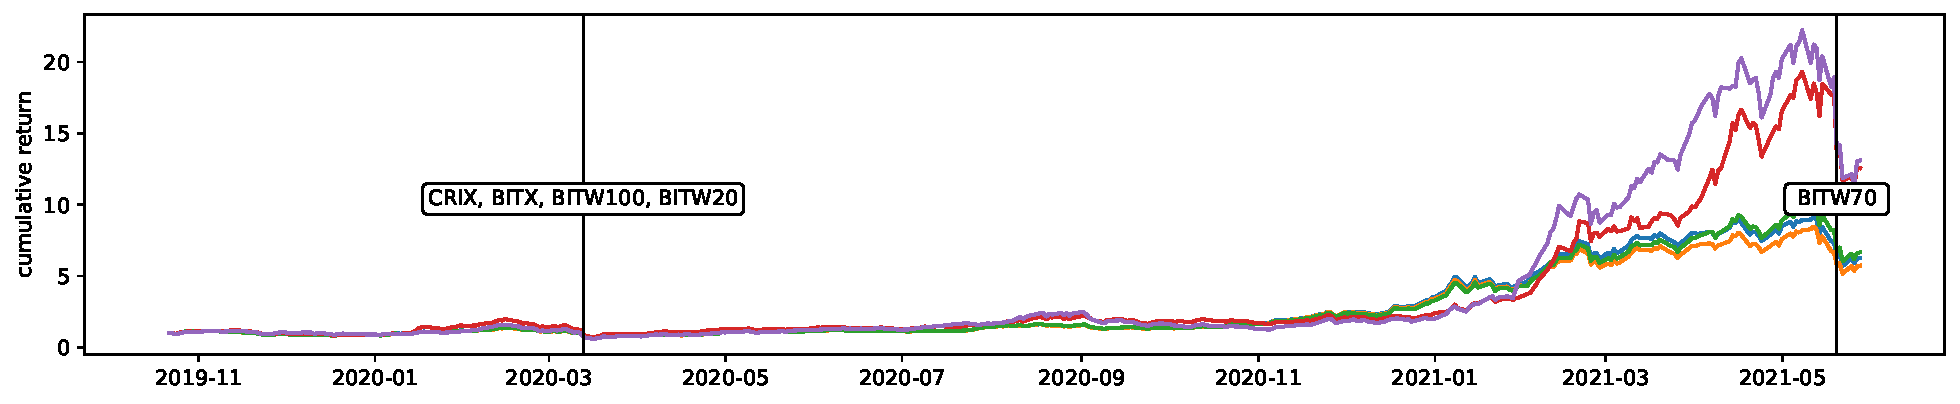
\includegraphics[width=\textwidth]{_pics/index_price.pdf}
  \caption{Out-of-sample cumulative returns of crypto indices. 
  The black vertical lines indicate the largest price drops of each
  index as indicated by the labels.
  The colouring is as follows:
  \textcolor{plt1}{Blue line} is CRIX;
  \textcolor{plt2}{Orange line} is BITX;
  \textcolor{plt3}{Green line} is BITW100;
  \textcolor{plt4}{Red line} is BITW20;
  \textcolor{plt5}{Purple line} is BITW70.
  }
%  \href{http://www.quantlet.com/}{\includegraphics[height=\baselineskip]{_pics/qletlogo_tr.png}} }
\label{fig:index_price}
\end{figure}

\begin{figure}[t]
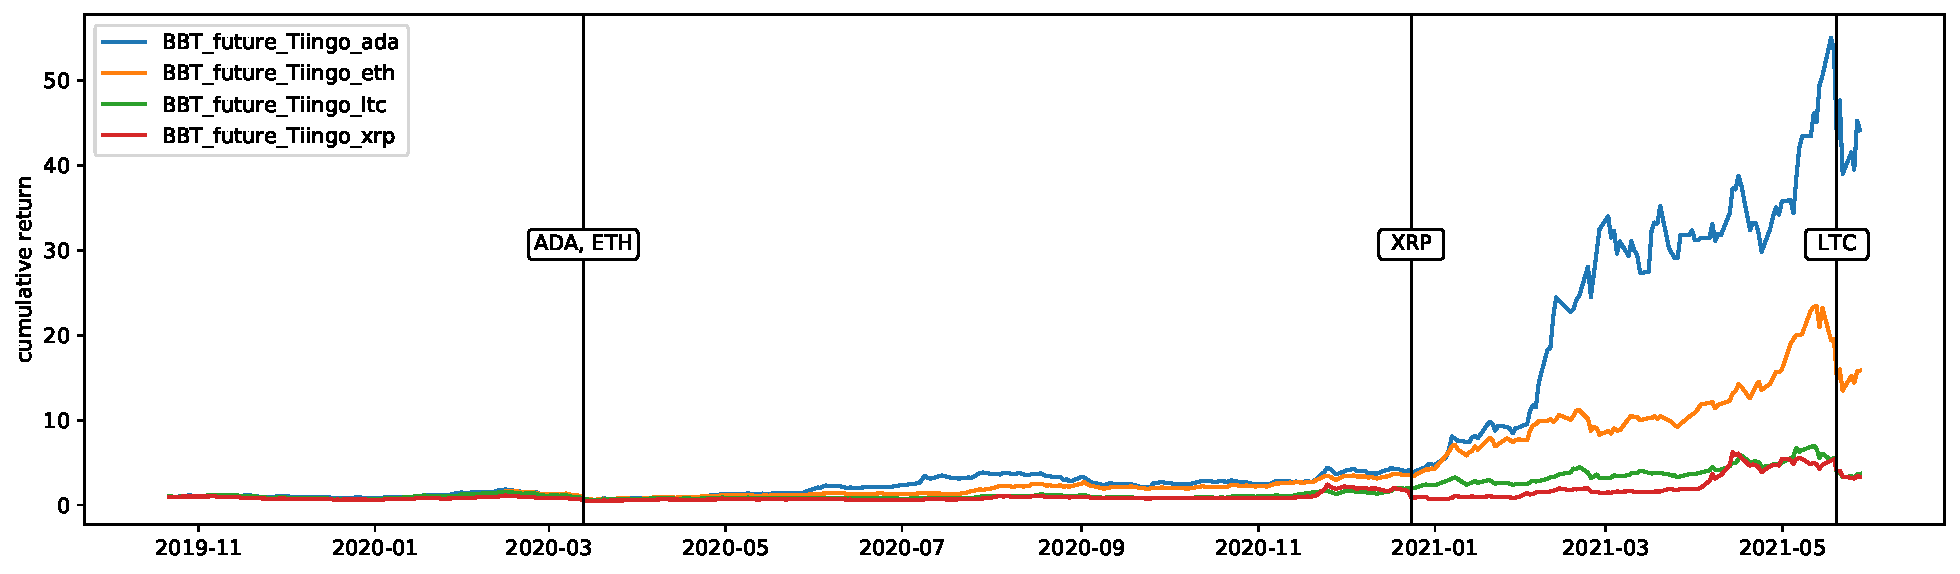
\includegraphics[width=\textwidth]{_pics/individualCoins_price.pdf}
  \caption{Out-of-sample cumulative returns of individual cyptos.
  The black vertical lines indicate the largest price drops each
  cryptos as indicated by the labels.
    \textcolor{plt1}{Blue line} is ADA;
  \textcolor{plt2}{Orange line} is ETH;
  \textcolor{plt3}{Green line} is LTC;
  \textcolor{plt4}{Red line} is XRP.}

%  \href{http://www.quantlet.com/}{\includegraphics[height=\baselineskip]{_pics/qletlogo_tr.png}} }
\label{fig:individualCoins_price}
\end{figure}

\begin{table}[t]
    \centering
      \begin{tabularx}{.8\textwidth}{cccX}
        \toprule
        Label &  Date & \% Drop in Price &  Summary\\
        \midrule
        CRIX    &2020-03-09 & 23.77 &
        \multirow[t]{6}{\hsize}{Coronavirus outbreak that affects the
          global markets including the crpyto market.}\\ 
        BITX    & & 23.68 &  \\
        BITW100 & & 23.87 &  \\
        BITW20  & & 26.66 &  \\
        ADA     & & 23.55 &  \\
        ETH     & & 27.40 &  \\
        BITW70  & 2021-05-19 & 27.64 & Spillover of the BTC shock on
        2021-05-17 (label A in Figure~\ref{fig:BTC_price} and
        Table~\ref{tab:BTC_5min})\\ 
        XRP     & 2020-12-23 & 41.00 & Top executives of Ripple Labs
        sued by the SEC of misleading investors$^1$. \\ 
        \bottomrule
      \end{tabularx}
        \caption{Summary of events that associated with largest price drops in out-of-sample data.
        The labels in the first column are the labels in Figure \ref{fig:index_price} and Figure \ref{fig:individualCoins_price}.
        CRIX, BITX, BITW100, BITW20, ADA and ETH have the same date
        the reason of the largest drop.$^1$ is reported by Bloomberg
        \url{https://bloom.bg/3cWdita}.} 
        \label{tab:All_min}
  \end{table}
\clearpage
\newpage
\subsection{An overview of the hedged portfolios without the copula
  selection step}
\label{subsec:HP1}
  \begin{figure}[t]
    \centering
    \begin{minipage}[t]{.475\textwidth}
        \centering
        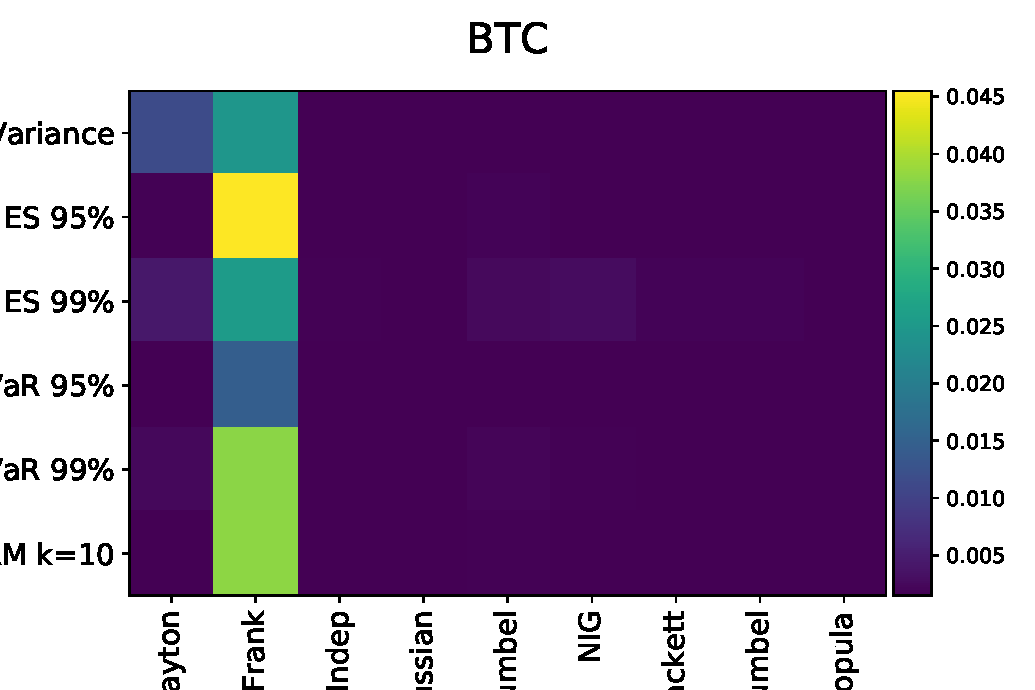
\includegraphics[width=\textwidth]{_pics/MSE_BTC.pdf}
      \caption{Out-of-sample mean square errors of BTC-BTCF portfolios constructed with different copula and risk minimization objectives.
        The Frank copula is inferior in the BTC-involved portfolios.}
    %    \href{http://www.quantlet.com/}{\includegraphics[height=\baselineskip]{_pics/qletlogo_tr.png}} }
    \label{fig:MSE_BTC}
    \end{minipage}
    \hfill
    \begin{minipage}[t]{.475\textwidth}
        \centering
        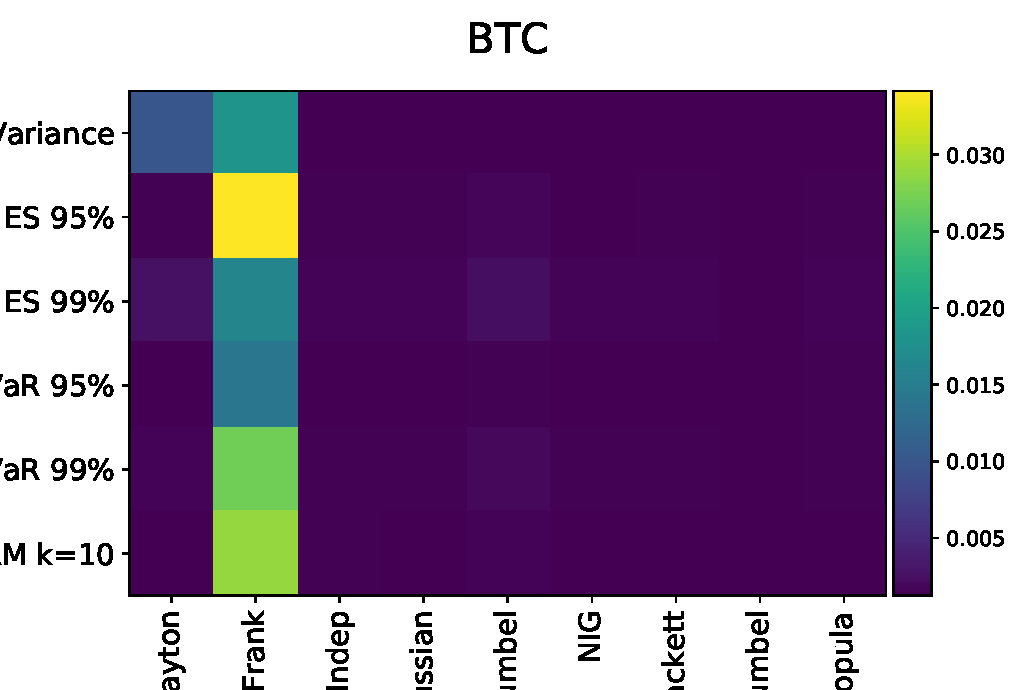
\includegraphics[width=\textwidth]{_pics/semiLowerVariance_BTC.pdf}
      \caption{Out-of-sample lower semivariance of BTC-BTCF portfolios constructed with different copula and risk minimization objectives.
      The Frank copula is obviously inferior.}
    %  \href{http://www.quantlet.com/}{\includegraphics[height=\baselineskip]{_pics/qletlogo_tr.png}} }
    \label{fig:SLV_BTC}
    \end{minipage}
    \end{figure}  

First, we analyse the results of the hedged portfolios without the
copula selection step in order to get a better understanding of how a
copula affects the hedged portfolio with various risk minimization
objectives.
To do so, we inspect the hedge performance of copulas by
the mean square error and lower semi-variance.
The mean square error
is the distance between a perfect hedge and the hedged portfolio
returns $\operatorname{MSE}= \E(R^2)$.
The lower semi-variance is defined as
$\operatorname{LSV}=\E \left( (R-\E(R))^2 \1_{\{R\leq \E(R)\}} \right)$.
All results presented here are out-of-sample results obtained without
the copula selection step in order to compare the performances across
copulae.

Figures \ref{fig:MSE_BTC} to \ref{SLV_indices} visualise the out-of-sample MSEs and LSVs of all the portfolios in colorplots.
Figures \ref{fig:MSE_BTC} and \ref{fig:SLV_BTC} are the MSEs and LSVs of BTC-BTCF. 
By far, the Frank copula is the worst performing copula.
In Figures \ref{MSE_indices} and \ref{SLV_indices}, the phenomenon
of Frank copula being inferior to its counterparts can also be observed
from the results of the CRIX, BITX, BITW100, and BITW20-BTCF
portfolios.
Interestingly, the spot in those portfolios usually have a strong
dependence with the BTCF.
In contrast, the inferiority of the Frank copula is less prominent in
the BITW70, ADA, ETH, LTC and XRP-BTCF portfolios.

We suspect that the Frank copula is not a choice to model assets with
strong dependence.

From Figures \ref{MSE_cryptos} and
\ref{SLV_cryptos}, one can see that the Gumbel copula is not performing as well as
other copulas in the ETH, LTC, and XRP-BTCF portfolios.
The reason is the Gumbel copula has only upper tail dependence,
while the ETH, LTC, and XRP exhibit lower tail dependence with BTCF.

\newpage
\begin{landscape}
\begin{figure}[h]
  \begin{minipage}[t]{0.475\linewidth}
    \centering
    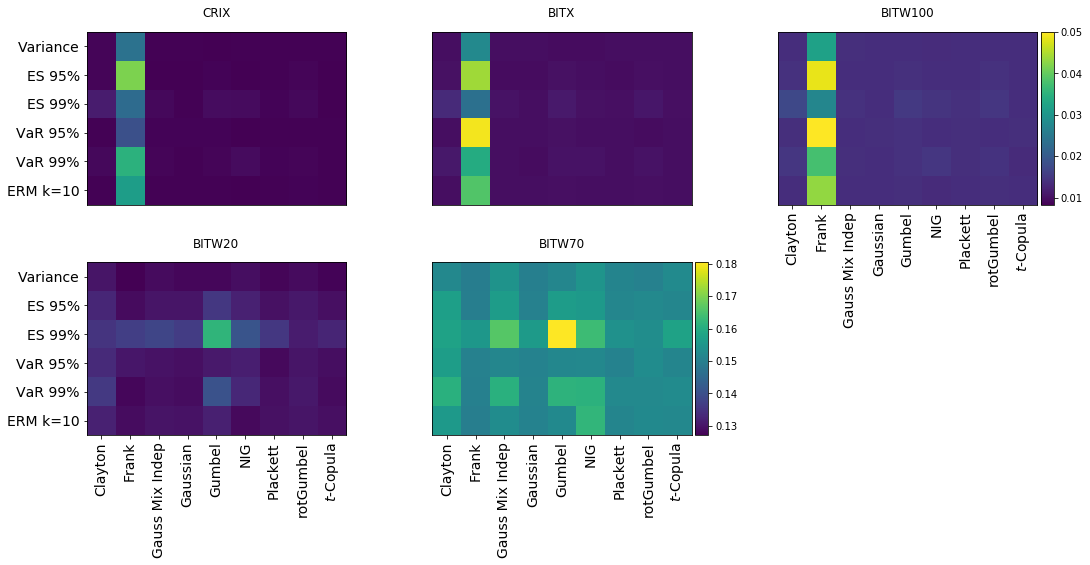
\includegraphics[height=.5\linewidth]{_pics/MSE_indices.png}
    \caption{Out-of-sample mean square errors of indices' hedge portfolios. Plots in a row share the same colour scale for comparison.}
    \label{MSE_indices}
  \end{minipage}
  \hfill
  \begin{minipage}[t]{0.475\linewidth}
    \centering
    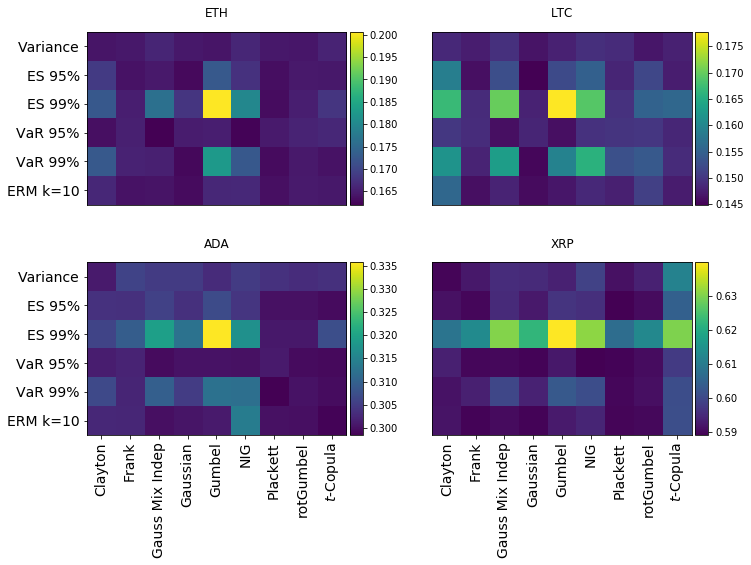
\includegraphics[height=.5\linewidth]{_pics/MSE_cryptos.png}
    \caption{Out-of-sample mean square errors of cryptos' hedge portfolios. Each plot has its own colour scale.}
    \label{MSE_cryptos}
  \end{minipage}
  \begin{minipage}[b]{0.475\linewidth}
    \centering
    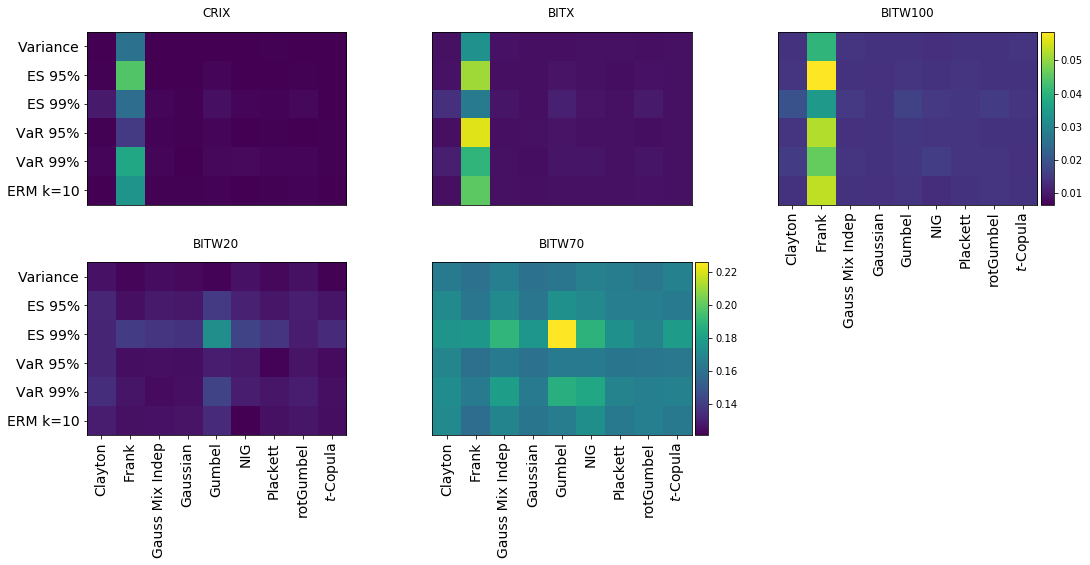
\includegraphics[height=.5\linewidth]{_pics/semiVariance_indices.png}
    \caption{Out-of-sample lower semi variance of indices' hedge portfolios. Plots in a row share the same colour scale for comparison.}
    \label{SLV_cryptos}
  \end{minipage}
    \hfill
  \begin{minipage}[b]{0.475\linewidth}
    \centering
    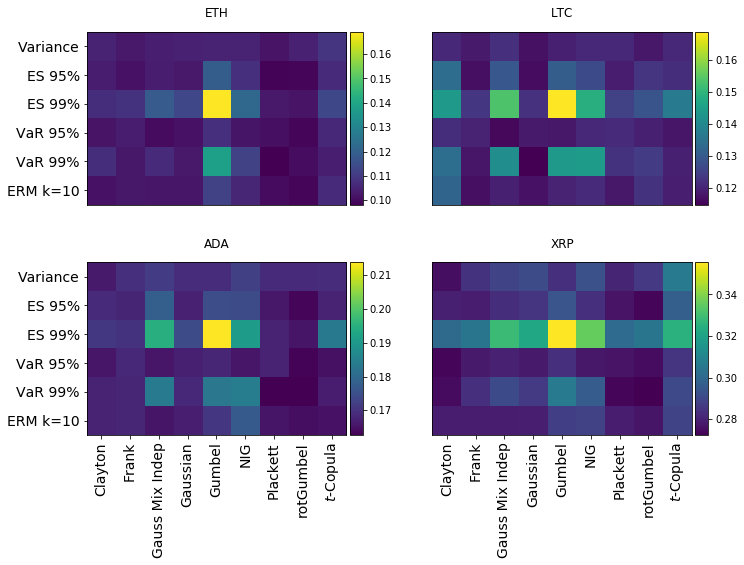
\includegraphics[height=.5\linewidth]{_pics/semiVariance_cryptos.png}
    \caption{Out-of-sample lower semi variance of cryptos' hedge portfolios. Each plot has its own colour scale.}
    \label{SLV_indices}
  \end{minipage}
\end{figure}
\end{landscape}

\subsection{Copula Selection Results}\label{subsec:-copula-results}
\begin{table}[t]
 \ra{1.1}
    {\begin{tabularx}{\textwidth}{lYYYYY} \toprule
         Copula/Asset & $t$ & Plackett & GMI & rotGumbel & NIG \\ \midrule
     \multicolumn{6}{l}{Individual Cryptos}                                                                                 \\
        \ \ \ BTC          & 73         & 4                 & 2                        & 1                  & 31                  \\
        \ \ \ ETH          & 3          & 6                 & 8                        & 94                 & 1                   \\
        \ \ \ ADA          & 0          & 0                 & 0                        & 0                  & 112                 \\
        \ \ \ LTC          & 13         & 0                 & 3                        & 32                 & 64                  \\
        \ \ \ XRP          & 0          & 31                & 3                        & 78                 & 0                   \\
   \multicolumn{6}{l}{Crypto Indices with BTC Constituent}                                                                  \\
        \ \ \ BITX         & 39         & 0                 & 14                       & 16                 & 12                  \\
        \ \ \ CRIX         & 47         & 0                 & 11                       & 3                  & 27                  \\
        \ \ \ BITW100      & 42         & 0                 & 8                        & 29                 & 2                   \\
    \multicolumn{6}{l}{Crypto Indices without BTC Constituent}                                                              \\
        \ \ \ BITW20       & 0          & 0                 & 0                        & 78                 & 3                   \\
        \ \ \ BITW70       & 0          & 0                 & 0                        & 80                 & 1                   \\
    \bottomrule
    \end{tabularx}
        \caption{Copula Selection Results. }









 \caption{Copula selection results (shortened).
        The values are the absolute frequencies of a copula chosen by
        the AIC procedure during the out-of-sample period. 
        Each frequenc represents five trading days, which corresponds
        to the recalibration interval.
        The table show the frequently chosen copulas, which are
        $t$, Plackett, Gaussian Mix Independent (GMI), rotated Gumbel
        (rotGumbel) and Normal Inverse Gaussian factor copula (NIG). 
        }
    \label{tab:copulasection}
\end{table}
Next, we inspect the copula selection results by the AIC procedure
described in Section~\ref{subsec:copula-selection}. 
Although the copula selection is only an intermediate step to obtain
the optimal hedge ratios,
the result of this step can help us better understand the dependence
feature between BTCF and the assets we study in this work.
This provides valuable information for modeling the assets in the future.
The decisions of the AIC procedure are summarised in Table
\ref{tab:copulasection}. Overall, the $t$-copula, rotated Gumbel
(rotGumbel), and the NIG factor copula are the most frequently chosen
copulae by the AIC procedure.

The $t$-copula is predominantly chosen by the AIC procedure to model the dependence between 
the BTC and BTC-involving-indices, CRIX, BITX, BITW100, and the BTC
future.
BTC and BTC-involving-indices exhibit strong (upper and lower) tail
dependence with BTCF, a strong tendency for one asset to be extreme when the other is extreme and
vice versa. 
See \cite{McNeil2015} for further details about tail dependence.
In fact, the $t$ copula has been recommended in various empirical
studies to model financial data, such as~\cite{zeevi2002beyond} and~
\cite{breymann2003dependence}.
Those studies suggest that the $t$-copula is a better model compared
to the Gaussian copula as financial data typically exhibit heavy tails
and tail dependence. 

% \natp{\em [I do not understand the argument with the radial
%   symmetry. Specifying the definition of radial symmetry is also not
%   helpful here. To sharpen the argument, it should be something like
%   this: On the other hand, the symmetry of the $t$-copula appears to
%   be a poor choice to model the remaining hedging pairs. Here, the AIC
%   criterion predominantly selects copulas that allow for asymmetry
%   between the spot and the underlying. This reflects that overall
%   dependence between a 
%   non-BTC-related spot asset and the BTCF may be low, but tail risk,
%   especially on the down-side is present, as crashes in the crypto
%   market, which occur frequently, do not differentiate between
%   assets.]} 
On the other hand, the symmetric $t$-copula appears to be 
a poor choice to model the remaining hedging pairs. 
\cite{demarta2005t} describes the symmetry feature of the $t$-copula ``strong'':
if $(U_1, ..., U_d)$ is a vector distributed in $t$-copula,
then $(U_1, ..., U_d) \overset{\mathcal{L}}= (1-U_1, ...,1-U_d)$.

Here, the AIC criterion predominantly selects copulas that allow for asymmetry between the spot
and the BTCF.
This reflects that overall asymetric dependence between a non-BTC-related spot asset and
the BTCF.
In fact, we observe from the crypto market that asset prices tend to crash simultaneously whereas positive development
tends to be idiosyncratic.   



Among the three popular copulae, rotGumbel copula shows its ability to
model the dependence between ETH and BTCF. rotGumbel also performs
well when modelling dependence between XRP, BITW20, BITW70, and the
BTCF. In particular, the whole time series of the two indices, BITW20
and BITW70, are best fitted solely with the rotated Gumbel
copula.

In fact, Clayton's AIC in many of the training sets is the second
lowest, just slightly higher than that of rotated Gumbel. This is because the
Clayton copula has the same ability to model the lower quantile
dependence. However, Clayton's radial like feature does not match the
behaviour of the financial data. 

It is worth to mention that although the NIG factor copula is
penalised heavily due to its three parameters setup, it is frequently
chosen to be the best copula to model the dependence between
individual cryptos and the BTC future. An extreme case occurs for ADA,
where only the NIG factor is chosen in our dataset. 
Another dependence structure best described by the NIG factor
copula is the pair of LTC-BTCF, with 64 out of 112 training sets best
fitted by the NIG factor copula. Indices like BITX and CRIX are
sometimes best fitted with the NIG factor copula as well, accounting
for modelling 12 and 27 training sets, respectively. 
The popularity of the NIG factor copula reflects the ability of the
copula to model complex dependence structure, involving heavier tails
than the Gaussian as well as asymmetric distributions.

%and
%off-diagonal (the region away from the diagonal line $(0,0)$ to
%$(1,1)$, see figure \ref{fig:copulaeScatterPlot}) behaviour. \natp{\em
%  [I think you did not understand my comment. It is clear what the
%  ``off-diagonal'' is. It is unclear what is meant by ``off-diagonal
%  behaviour''. Do you mean extremes on the other diagonal? Do you mean
%  a cloud of points away from the diagonal? Not sure what the NIG
%  factor copula is capable of modelling in this respect. Perhaps you
%  have a reference?]}

The Frank copula turn out to generally be a poor choice to model financial
data (as also reported by \cite{barbi2014copula}).
The Plackett copula is characterised by its dependence parameter being
equal to the cross-product ratio, see
(\ref{eq:PlackettCrossProduct}). However, this property
does not capture the dependence structure of cryptos and BTCF.

\subsection{Hedged portfolios with the copula selection step}\label{subsec:HP2}

\afterpage{
  \begin{landscape}
  \begin{table}[!] \centering
\resizebox{.8\paperheight}{!}{%
\begin{tabular}{l*{10}{r}}
\toprule
{} &   BTC & ETH & ADA & LTC & XRP & BITX & CRIX & BITW100 & BITW20 & BITW70\\
\midrule
  \multicolumn{10}{l}{Spots assets only}   \\
\ \ \ Mean \%  &      0.3915 &      0.6819 &      0.9467 &      0.3227 &      0.2987 &      0.4308 &      0.4602 &      0.4683 &      0.6249 &      0.6353 \\
\ \ \ Std \%   &      4.4023 &      6.0103 &       6.699 &      6.4781 &      7.9843 &      4.5676 &       4.542 &      4.6174 &      5.5021 &      5.8155 \\
\ \ \ MD \%    &    -25.9965 &    -32.0144 &    -26.8528 &    -37.5913 &    -52.7652 &     -27.022 &    -27.1385 &    -27.2694 &    -31.0092 &    -32.3453 \\
\ \ \ MD date &  2020-03-12 &  2020-03-12 &  2020-03-12 &  2021-05-19 &  2020-12-23 &  2020-03-12 &  2020-03-12 &  2020-03-12 &  2020-03-12 &  2021-05-19 \\
  \multicolumn{10}{l}{Variance minimizing portfolios}   \\
\ \ \ Mean \%  &      0.0215 &      0.2823 &      0.5617 &     -0.0871 &     -0.0123 &      0.0561 &      0.0812 &      0.0855 &      0.2429 &      0.2706 \\
\ \ \ Std \%   &      0.3221 &      3.8741 &      5.2722 &      3.9052 &      7.1537 &      0.9954 &      0.9183 &      1.1986 &      3.5846 &      3.8838 \\
\ \ \ MD \%    &     -1.4393 &    -17.7421 &    -13.8687 &    -28.3029 &    -52.5236 &     -7.7567 &     -7.1025 &    -11.3866 &     -21.468 &    -23.9984 \\
\ \ \ MD date &  2020-11-30 &  2021-05-19 &  2021-01-08 &  2021-05-19 &  2020-12-23 &  2021-05-19 &  2021-05-19 &  2021-05-19 &  2021-05-19 &  2021-05-19 \\
  \multicolumn{10}{l}{VaR 95\% minimizing portfolios}   \\
\ \ \ Mean \%  &      0.0253 &      0.3084 &      0.5726 &     -0.0742 &      0.0208 &      0.0562 &      0.0863 &      0.0846 &      0.2728 &      0.2847 \\
\ \ \ Std \%   &      0.3294 &      3.8944 &      5.2204 &      3.9145 &       7.152 &       0.993 &      0.9151 &       1.198 &       3.594 &      3.9133 \\
\ \ \ MD \%    &     -1.5347 &     -19.175 &    -14.6974 &    -28.3672 &    -52.5667 &     -7.5639 &     -6.9744 &    -11.2582 &    -22.0733 &    -24.6513 \\
\ \ \ MD date &  2020-11-30 &  2021-05-19 &  2021-05-19 &  2021-05-19 &  2020-12-23 &  2021-05-19 &  2021-05-19 &  2021-05-19 &  2021-05-19 &  2021-05-19 \\
  \multicolumn{10}{l}{VaR 99\% minimizing portfolios}   \\
\ \ \ Mean \%  &      0.0176 &      0.2977 &      0.5562 &     -0.0852 &      0.0352 &      0.0593 &      0.0738 &      0.0823 &      0.2499 &      0.2788 \\
\ \ \ Std \%   &       0.327 &      3.9132 &      5.3466 &      4.1503 &      7.1658 &      1.0178 &      0.9695 &      1.2338 &       3.621 &      3.9257 \\
\ \ \ MD \%    &     -1.5689 &    -18.6061 &    -15.4795 &    -29.0915 &    -52.5727 &     -8.0299 &     -7.0185 &    -11.8752 &    -21.6634 &    -24.5294 \\
\ \ \ MD date &  2020-11-30 &  2021-05-19 &  2021-05-19 &  2021-05-19 &  2020-12-23 &  2021-05-19 &  2021-05-19 &  2021-05-19 &  2021-05-19 &  2021-05-19 \\
  \multicolumn{10}{l}{ES 95\% minimizing portfolios}   \\
\ \ \ Mean \%  &      0.0204 &      0.3082 &      0.5525 &     -0.0808 &      0.0176 &      0.0591 &      0.0777 &      0.0848 &      0.2608 &      0.2785 \\
\ \ \ Std \%   &      0.3234 &       3.889 &      5.2673 &      3.9829 &      7.1533 &      1.0065 &      0.9207 &      1.2125 &      3.6115 &      3.9157 \\
\ \ \ MD \%    &     -1.5629 &    -18.7819 &    -14.9647 &    -28.4608 &    -52.5698 &     -7.6211 &     -6.9894 &    -11.1357 &     -21.543 &    -24.3474 \\
\ \ \ MD date &  2020-11-30 &  2021-05-19 &  2021-05-19 &  2021-05-19 &  2020-12-23 &  2021-05-19 &  2021-05-19 &  2021-05-19 &  2021-05-19 &  2021-05-19 \\
  \multicolumn{10}{l}{ES 99\% minimizing portfolios}   \\
\ \ \ Mean \%  &      0.0148 &       0.308 &      0.5016 &     -0.1029 &       -0.02 &      0.0598 &      0.0835 &      0.0781 &      0.2538 &       0.266 \\
\ \ \ Std \%   &      0.3476 &      3.8954 &       5.404 &      4.1581 &      7.2887 &      1.0312 &      0.9461 &       1.264 &      3.6323 &       3.932 \\
\ \ \ MD \%    &     -1.6225 &    -18.7625 &    -15.4481 &    -29.1727 &      -52.57 &     -7.7424 &     -7.0203 &    -11.9263 &    -21.9866 &    -24.4764 \\
\ \ \ MD date &  2020-11-30 &  2021-05-19 &  2021-05-19 &  2021-05-19 &  2020-12-23 &  2021-05-19 &  2021-05-19 &  2021-05-19 &  2021-05-19 &  2021-05-19 \\
  \multicolumn{10}{l}{ERM $k=10$ minimizing portfolios}   \\
\ \ \ Mean \%  &      0.0223 &      0.3117 &      0.5722 &     -0.0512 &      0.0155 &       0.059 &       0.084 &      0.0853 &      0.2564 &      0.2818 \\
\ \ \ Std \%   &      0.3221 &      3.8679 &       5.359 &      3.8812 &      7.1579 &      1.0078 &      0.9087 &      1.2032 &      3.6009 &      3.9074 \\
\ \ \ MD \%    &     -1.5242 &    -18.8729 &    -14.3885 &    -28.0879 &    -52.5689 &     -7.8581 &      -7.053 &    -11.1846 &     -21.592 &     -24.525 \\
\ \ \ MD date &  2020-11-30 &  2021-05-19 &  2021-01-08 &  2021-05-19 &  2020-12-23 &  2021-05-19 &  2021-05-19 &  2021-05-19 &  2021-05-19 &  2021-05-19 \\
\bottomrule
\end{tabular}}
\end{table}
\end{landscape}
}

We now turn to the hedge performance. 
Table~\ref{tab:bigTable}
presents the first two moments, maximum drawdown (MD) and the date of
MD of the hedge portfolios. An interesting observation is the similarity of
the statistics when minimising with respect to different risk measures.
Detailed statistics are in Tables~\ref{tab:var_rh} to \ref{tab:ERM_rh} in Appendix
\ref{appendix:summary_stats}. 
 
Unsurprisingly, the BTC-involved spots, i.e., BTC, CRIX, BITX, and
BITW100, are well hedged by the BTCF regardless of risk minimization
objective. 
The BTC-not-involved spots, on the contrary, are less promising. Those
hedge portfolios' returns are nearly as volatile as the
assets themselves, see for example ADA and XRP. 
We further discuss the effectiveness of hedge in the next
section. %\ref{sec: HE results}. 

\subsection{Hedging Effectiveness Results}\label{sec: HE results}
In this section, we analyse the out-of-sample hedging effectiveness
(HE) of BTCF as a hedge instrument. 
HE is defined as $$\text{HE} = 1-\frac{\rho_h}{\rho_s},$$
i.e., it measures the percentage reduction of risk of the hedge
portfolio $\rho_h $ relative to the risk of the spot position $\rho_s$.
A higher HE indicates a greater risk reduction and thus the hedge is
more effective.  
The HE above is a generalisation of how \citet{ederington1979hedging}
evaluates hedge performance, which focusses on variance as the risk
measure. 
Aside from variance, we include the risk measures which act as
loss function while searching for the optimal hedge ratios: ES 95\%
and 99\%, VaR 95\% and 99\% and ERM.

\begin{figure}[t]
  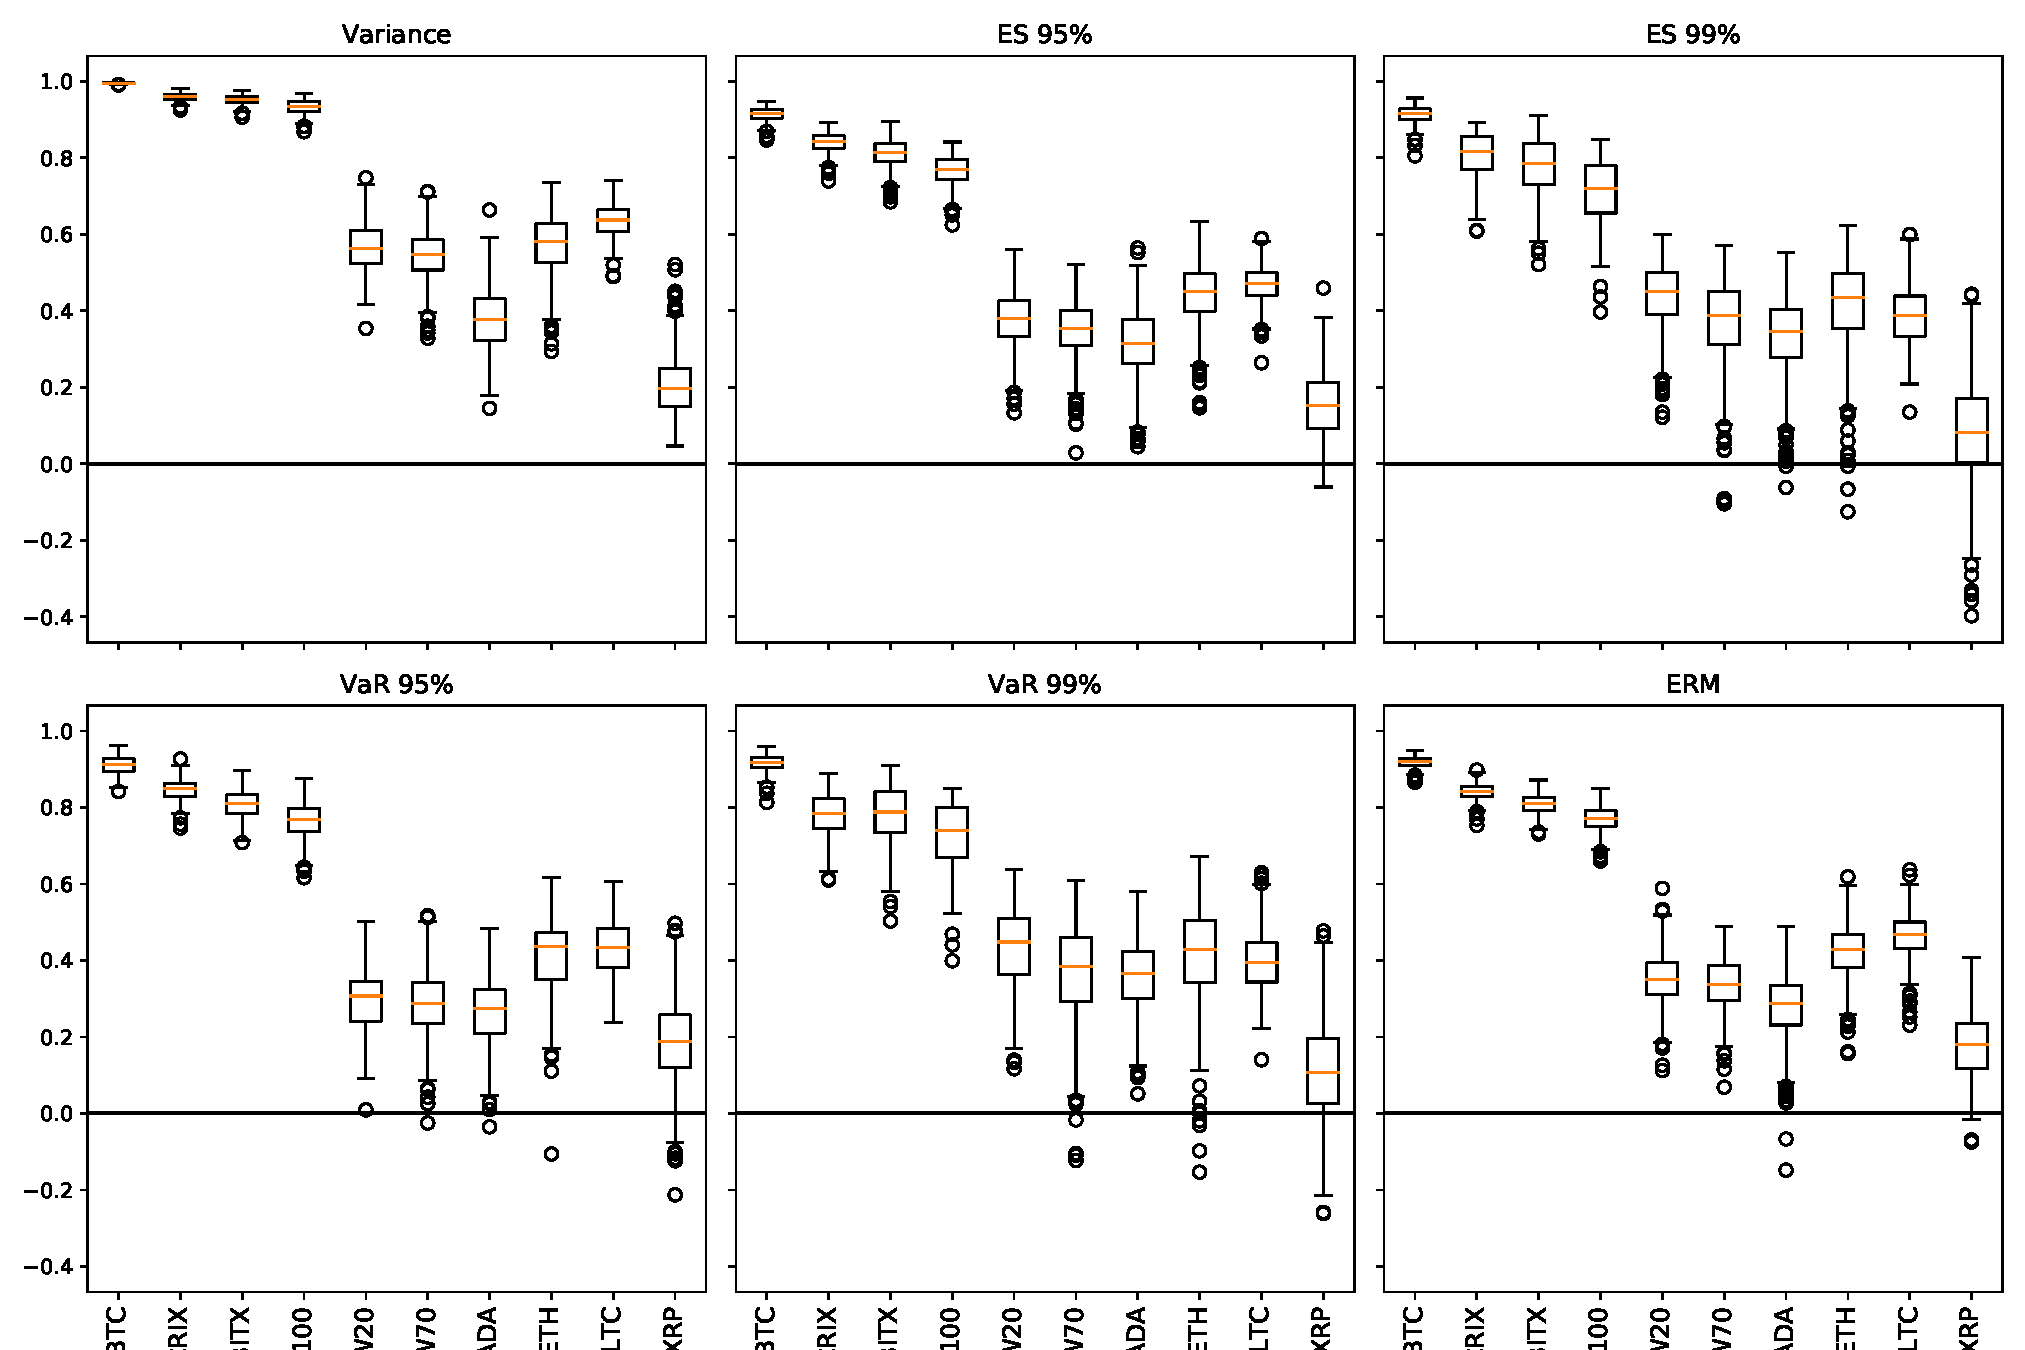
\includegraphics[width=\textwidth]{_pics/HE_boxplot.pdf}
    \caption{Hedging effectiveness (HE) of portfolios with different risk minimization objectives evaluated by the corresponding risk minimization objectives.
              The boxplots indicate the the median, upper quartile, lower quartile, minimium and maximum of the bootstrapped HE.
              The HE of BTC-involved spots are significantly higher than that of BTC-not-involved spots.
    \href{http://www.quantlet.com/}{\includegraphics[height=\baselineskip]{_pics/qletlogo_tr.png}} }
  \label{fig:HEboxplot}
  \end{figure}

% \natp{\em [A description is missing of how the hedge actually
%   works. How much data enters the calibration (I believe it's 300
%   days). Then what happens? On each day we have a hedge ratio. Do we
%   construct a new hedge each day? How long is the hedge period? So,
%   after which time period is P\&L calculated. 
%   This could also be added to Section 2.2.\\
%   What is the motivation behind the bootstrapping?]}


As described in Section \ref{sec:empirical-procedure}, the backtesting procedure gives
an out-of-sample hedged portfolio return time series for every spot-copula-risk measure combination. 
The time series represent the profit and lost if hedgers recalibrate copulae and adjust the hedge ratio every 5 days.  
In order to obtain a robust HE result (instead of a point estimate), we apply the bootstrapping method.
Bootstrapping refers to sampling from the empirical distribution of a
given data sample (e.g.\ a time series of fiancial returns). The
principal idea underlying bootstrapping is to provide statistical
information about estimators that cannot be derived from just one
realisation of the data. The method was introduced by
\cite{Efron1979}; see also \citep{efron1994introduction, davison1997bootstrap}. 

A specific type of bootstrapping method designed for timeseries, namely the stationary block bootstrap \cite{Politis1994}, is applied in our analysis.
The stationary bootstrapping procedure is as follows. 
Assume a time series $\{X_t\}_{t \in [1,N]}$ that is
a stationary weakly time dependent time series,
 we first draw a block of samples $\{X_i, ..., X_{i+j-1}\}$, where the index $i$ is a
random variable uniformly distributed over 
$[1,2,...,N]$ and $j$ is geometric distributed random variable with
parameter $p$ independent of $i$. 
For any index $k$ which is greater than $N$, the sample $X_k$ is
defined to be $X_{k(\mathrm{mod} N)}$. 
Then, we repeat the procedure until the number of samples are drawn in total across the blocks equal or exceed a predefined sample length $S$. 
One bootstrapped time series sample is then the concantenation of the blocks truncated to length of $S$.
The resulting bootstrapped time series is known as pseudo time series. 

% For each block, we calculate the hedging effectiveness as outlined above.
We choose $p=1/5$, implying the average block length is 5 such that it aligns with the recalibration frequency. 
The length of each pseudo time series sample $S = 300$ is chosen to be aligned with the length of each training set.  
The length of each pseudo time series sample allows ES and VaR to be calculated in a reasonable length.
We draw in total $n=500$ pseudo time series,
for each of them we compute various HE measures to obtain a collection of HE samples. 

% 100 blocks are drawn for each risk minimising objective and
% spot. 

%\natp{\em [You need to go over this again. There are many
%  grammatical errors in there that need to be fixed. Also explain that
%  expected block length is 200 so that ES99\% and VaR99\% can be
%  calculated. Is the hedge ratio calculated for each sample drawn,
%  etc.? ]}

% \natp{\em [The previous part still needs quite a bit of work as it
%   remains unclear to the reader what is actually going on. The
%   principal idea is to create an out-of-sample distribution of HE, but
%   with one sample path this is not possible. Therefore, the bootstrap,
%   right?]}

Figure \ref{fig:HEboxplot} reports the bootstrapped HE samples.
As expected, the BTC involving spots, the BTC, CRIX, BITX and BITW100, are well hedged
by the BTCF. 
The HEs of the other cryptos and indices are
substantially lower than to the BTC-related instruments, but 
exhibit a consistent performances across different risk measures. 
As it turns out, some HE bootstrapping samples are even negative,
which means the ``hedge'' portfolio actually increases the risk. 
This shows BTC futures is not suitable for cross-asset hedges (cross hedge).

%\natp{\em[It does not
%  make sense to compare across different risk measures, so I suggest
%  to delete the last statement. }

%\natp{[How can HE be negative??? Especially
%  for variance this is impossible.]}

%\natp{\em [We need some proper conclusions here.
%  \begin{itemize}
%  \item It is noticable that the HE of variance is highest.
%  \item Comparing ES95\% and ES99\%, it is seen that ES95\%
%    performs better. This is an indication that tail risk remmains
%    despite hedging.
%  \end{itemize}
%  ]}



%\natp{\em [A general conclusion is needed. That ES95\% / Var95\%
%  perform better than their 99\% counterparts is also evident from
%  Figures 7 and 8. So focussing on tail risk by choosing an extreme tail risk
%  measure does not lead to a promising hedge. Also variance performs
%  well, especially for the lower correlated instruments /
%  indices. Var95\% also performs well across all copulas. Please check
%  if the tables in the appendix confirm this.\\
%  Main conclusion is that the choice of copula highlights the
%  differences in the instruments / indices and their relationships
%  with the futures contract. Unfortunately, we see that the copula
%  choice does not always lead to the best hedge (see e.g.\ ADA), where
%  Frank, Gaussian, Plackett and rotGumbel perform much better in
%  terms of MSE. I suspect that has to do with the fact that hedging is
%  necessarily linear, so a better copula model may not necessarily
%  attain a better (linear) hedge. This means that the copula selection
%  results should be taken as interesting by themselves. Also, they
%  might be useful if using more than one hedge instrument, e.g.\ by
%  including options as hedge instruments.]}

%%% Local Variables:
%%% mode: latex
%%% TeX-master: "SRM"
%%% End:
